\documentclass[tikz]{standalone}

\usepackage{tikz}
\usetikzlibrary{arrows,decorations.pathmorphing,backgrounds,positioning,fit,petri}

\begin{document}
  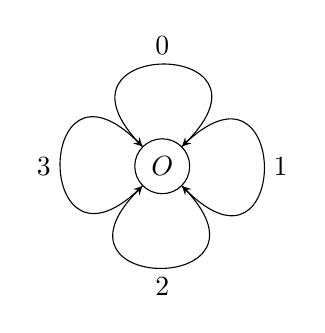
\begin{tikzpicture}[>=stealth]% Example:
  \node (o) at (0,0) [circle,draw] {$O$};
  \draw [->] (o) to[
      out=135, in=45, looseness=10,
      edge node={node [sloped, above] {$0$}}
    ] (o);
  \draw [->] (o) to[
      out=45, in=-45, looseness=10,
      edge node={node [right] {$1$}}
    ] (o);
  \draw [->] (o) to[
      out=-45, in=-135, looseness=10,
      edge node={node [below] {$2$}}
    ] (o);
  \draw [->] (o) to[
      out=-135, in=-225, looseness=10,
      edge node={node [left] {$3$}}
    ] (o);
  \end{tikzpicture}%
\end{document}